\section{Introduction}

Android allows developers to write native code that is able to interact with the Java code. This can be accomplished with the Native Development Kit (NDK). In the documentation of the NDK it is stated, that the NDK can be useful in the following cases \cite{AndroidNdkIntro}

\begin{itemize}
	\item Squeeze extra performance out of a device to achieve low latency or run computationally intensive applications, such as games or physics simulations.
	\item Reuse your own or other developers' C or C++ libraries. 
\end{itemize}

In \cite{5669738} it was shown that the use of native code can speed up Java applications considerable.

As stated in \cite{AndroidNdkIntro} , the communication between Java and the native code is done via Java Native Interfaces(JNI) \footnote{\url{https://docs.oracle.com/javase/8/docs/technotes/guides/jni/spec/jniTOC.html}}. 
JNI is a native programing interface, so that Java code running in the JVM can interoperate with applications and libraries written in other programming languages \cite{JNISpecChapter1}.

JNI wasn't designed with security in mind and doesn't do any security checks. This fact can be derived from the design specification document from JNI (section 'Reporting Programming Errors')\cite{JNISpecChapter2}.
The native code has direct access to the memory of the running process and
as the Java and native code are running in the same memory address space, the native code is able to read and write arbitrary memory from the JVM \cite[p. 2]{Afonso2016GoingNU}.

It can be registered, that JNI is a powerful tool that doesn't restrict the developer. On the one side this speeds up execution of native code and is convenient for developers, but on the other side it is also very dangerous seen from a security perspective.
If an attacker is able to execute code in a native library the executed code can abuse the power of JNI, too.\\

A selection of possible attacks exploiting JNI are:
\begin{itemize}
\item As native libraries reside in the same address space as a JVM, bugs in native
libraries can enable attackers to read and write the JVM's memory \cite[p. 3]{Sun_jvm-portablesandboxing}. %\textbf{TODO:} Mention example attack
	\item  Similar to the Reflection API, JNI allows to retrieve and set the content of private fields. This enables an attacker to steal confidential information \cite[p. 3]{Sun_jvm-portablesandboxing}.
	\item JNI allows to set the destination of an object pointer without type-checking. Thus type-confusion attacks are possible \cite[p. 4]{Sun_jvm-portablesandboxing}. %\textbf{TODO:} What can be achieved by type confusion attacks?
	\item Bugs in the Linux kernel can enable an attacker to escalate privileges, like done in 'Dirty Cow' (CVE--2016--5195) \cite{DirtyCow}. Over JNI such attacks can directly be initiated
    \item Changing the behavior of the Java application by replacing functions by manipulating or injecting byte code using code patching methods.
	\item Changing the behavior of the Java application by replacing functions by manipulating or injecting byte code using code patching methods.
	We will present later in this paper an example for this kind of attack.
\end{itemize}

It should be highlighted that quite a few Android apps use native code: In a survey of Google Play apps \cite[p. 3]{Sun:2014:NPA:2627393.2627396} it was found out, that 86\% of the top 50 apps have been shipped with native code. It was also stated, that there were also apps (like Skype), that use native code for a common core being shared among multiple platforms. If an app would be compromised through a flaw in the native code, possible thousands or even millions of systems would be affected, thus these apps could be an interesting target for attackers. \\

In this paper we will analyze how the security vulnerabilities exposed by JNI can be abused by an attacker, if he is able to execute code in a native library, and how the attacker can compromise the benign target app using native code.

The following sections of this paper are structured as follows: In Section 2 we will look at other works dealing with security concerns of native code, in Section 3 we will discuss techniques and methods we will need for Section 4, where finally the aforementioned attack scenario is presented. 

%\textbf{TODO:} Describe shortly the method for the attack scenario

\section{Related work}

Until 2014, the security threats coming from native libraries wasn't given that much attention since it was mistakenly believed that native code would be as secure as Java code since Android regulates all components above the kernel \cite[p. 1]{Sun:2014:NPA:2627393.2627396}. \\
But in recent years, more effort was done in finding ways to make native library calls more secure.

In \cite{Afonso2016GoingNU} the authors analyzed dynamically about of 446 thousand Android apps that use native code and developed a Native-Code policy that limits many malicious behaviours while still allowing the correct execution of 99.77\% of the benign apps.

The authors from \cite{Sun:2014:NPA:2627393.2627396} present a security framework called NativeGuard, that isolates and executes code from native libraries in a separated non-privileged application. The communication with the source app is done via interprocess communication. Through NativeGuard, native libraries don't inherit privileges from the Android app and they cannot access the memory from it anymore.  
Also a well known software sandboxing project is Robusta \cite{Siefers:2010:RTN:1866307.1866331}. %\textbf{TODO: More Description}

Not explicitly designed for Android, but nevertheless an interesting project is CHERI JNI, that is a hardware-assisted implementation of JNI extending the guarantees required for Java's security model to native code \cite{Chisnall:2017:CJS:3093337.3037725}.

In \cite{ExecuteThis} the security implications of loading additional code from external sources at runtime have been analyzed. Attackers can abuse the code loading to hide malicious code from security services like Google Bouncer. But benign applications can also have vulnerabilities, if the code loading is done insecurely. It was found out, that Android doesn't enforce enough security checks on external code and developers of benign apps often don't implement right appropriate protection mechanisms or are unwitting of the threats. The authors have done a large-scale analysis of popular Google Play apps and have laid bare that 9.25\% of them are vulnerable to code injection attacks. As a sample attack they did a HTTP Man-In-The-Middle attack (MITM) on a benign application:
They exploited an insecure http connection. The stated app had implemented an update process where the update was downloaded from a remote HTTP server. The update is then loaded through a Classloader at runtime. But by using the insecure HTTP connection instead of HTTPS, the application is vulnerable to a MITM attack, through which again an attacker could execute arbitrary code that is allegedly considered to be an update.
With the results of the analysis they modified the Dalvik VM in such a way that attacks through external code loading can be blocked. They did this by adding missing security checks for external sources.

Most of the apps out there are free apps, as shown in \cite[p. 164]{Wang:2017:ESM:3038912.3052712}, that 15\% of all Android apps are paid apps, however they only account for 0.2\% of the total app installs. 
Thus, it is not surprising that the developers of free apps like to use advertising libraries: A survey of 2012 showed that 49\% of all apps and 50\% of the top free apps used libraries for monetarized advertising \cite[p.7]{Pearce:2012:APS:2414456.2414498}. 
Advertising libraries have a large user base and thus security plays even a major role. 
If an advertising library gets compromised through a malicious insider or a flaw in the native code, this could guide to fatal consequences. 
An actually well-intentioned C code could lead through memory safety vulnerabilities to arbitrary code injection as elaborated in \cite{Szekeres:2013:SEW:2497621.2498101}.

\section{Background}

In this section we look at some background knowledge that is necessary to understand the attack scenario that we will present in the next section.
%In this section we want to examine how an attacker could manage it so that malicious (native) code gets executed. Of course the bandwidth of possible attacks is much too large, so we want pick out some interesting attacks shining out. 
 
\subsection{Java Native Interface}

Loading a native library from Java can be accomplished by:
\begin{lstlisting}[language=Java, style=JavaCodeStyle]
 System.loadLibrary("libName");
\end{lstlisting}
Where \emph{libName} is the name of the native library without file extension since the file extension is platform dependent.

The declaration of a native method is done in Java as well. It resembles the declaration of an interface method, but uses the 'native' keyword:
\begin{lstlisting}[language=Java, style=JavaCodeStyle]
package com.example;
public class Native {
  public native String fromNative();
}
\end{lstlisting}

The definition of  a native method is done using native code (here C++). This example defines a native method, that returns a \emph{java.lang.String} class object.
\begin{lstlisting}[language=C++, style=CppCodeStyle]
extern "C" JNIEXPORT jstring JNICALL
Java_com_example_fromNative(JNIEnv *env,jobject /* this */) {
    const char* msg = "Hello from C++";
    return env->NewStringUTF(msg);
}
\end{lstlisting}

Over the JNIEnv variable \emph{env}, the C programer can access the methods of the JNI interface. The JNIEnv variable is created by the JVM. Before the native function is called, a pointer to the JNIEnv variable is pushed on the callstack as the first parameter. The second argument of type jobject is a pointer to the java object the native method is called from. For static native methods, a pointer to the class the native method belongs to, is pushed instead. 

\subsection{Android Runtime (ART)}
In Android, currently there exist two Virtual machines: The older solely JIT-compiling Dalvik and the newer one: ART. ART introduced Ahead-of-time compilation (AOT) in Android \cite{ArtAndDalvik}. AOT precompiles the majority of the java code on install time, which speeds up program starts of apps. ART replaced Dalvik in Android 5.0 (Lollipop) \footnote{\url{https://developer.android.com/about/versions/android-5.0-changes.html}}. For that reason, we will design our attack scenario exploiting ART internals, as Dalvik isn't used anymore in newer Android versions. But it should be noted, that a similar attack would be possible for the Dalvik runtime.

In Android 7.0 (Nougat) a JIT Compiler was again reintroduced that works along with the AOT compiler \cite{Android7ForDevelopers}. The reason for this were to improve runtime performance, saving storage space and speeding up application and system updates \cite{JitWorkFlow}.

On a simplified view, the new JIT-Compiler basically works like follows:  


\begin{itemize}
    \item Only 'hot' methods are compiled Ahead-of-time 
    \item A method is 'hot' if it is called often.
    \item On install time an analyzing process decides which methods are likely to be 'hot'.
    \item On runtime, the Analyzer checks regularly if a method is 'hot'
    \item If a method gets 'hot', it will be compiled by the AOT compiler
    \item Native methods are not interpreted, they never will get hot \newline
    \textcolor{red}{TODO: Proceed here!}
    $\Rightarrow$ In order to replace an existing java method, the method has to be set to native and its 'hotness' count has to be set to 0 (not 'hot')
    \end{itemize}
    
In figure \ref{JitWorkflow} we see how the new JIT compilation works starting from Android 7.0.     
    
\begin{figure}[H]
	\begin{center}
	%\vspace*{-0.1cm}
		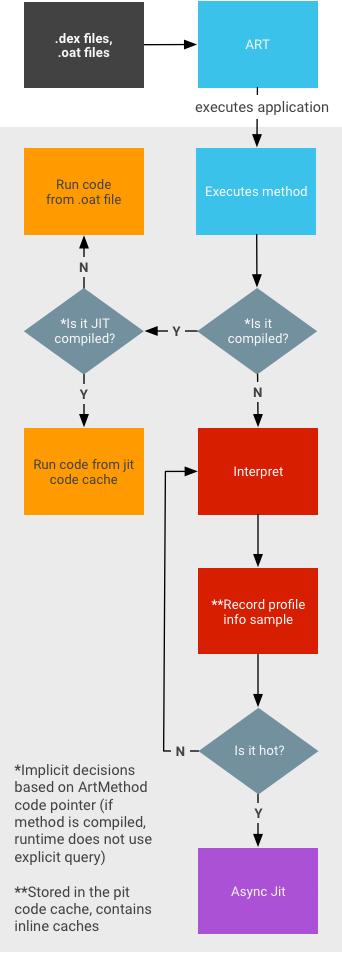
\includegraphics[scale=0.45]{figures/jit-workflow-extract.png}
	\end{center}
	\caption{Extract from the JIT Workflow on Android 7.0 and above \cite{JitWorkFlow}}
	\label{JitWorkflow}
\end{figure}

When compiling an android app, the Java source files get compiled first to *.class files as usual and then compiled to Dalivk bytecode. The resulting code is stored into a  Dalvik Executable (DEX) file and finally packed into an Android Package Kit (APK). This process is independent from the later VM the target device uses.

Now we assume on the target device is installed Android 7.0 or above.
While installing the app, ART analyzes the *.dex files and optimizes the code. As a result of this optimization step, 'hot' methods get AOT compiled and stored in *.oat files, that are binary files for AOT compiled methods.


When an Android app starts, the corresponding *.dex and *.oat files get loaded to memory by ART. The JIT-compiler checks upon the calling of a method, whether the method is compiled or not. If the method is compiled, it is further checked, whether the compiled method is AOT-compiled or JIT-compiled. The result of the checks determines, whether the method is run from the *.oat file or from the JIT code cache.

Should the method to be executed not be a compiled method, it is going through several steps: At first it is executed by the interpreter, than a profile sample is recorded and as the last step it is checked, whether the method is 'hot'. If the method is not 'hot', its hotness counter is incremented. 
If the method is 'hot' the method is (asynchronously) JIT compiled. 

\section{Attack Scenario}
In this section we will present and discuss a possible attack from native code, that leverages the power of memory insecurity in C++ to compromise an Android Java application. The content of this section is structured as follows: In Subsection \emph{\textbf{Model}} we present the theoretical concept of the attack, some design decisions and the demo application. 
In Subsection \emph{\textbf{Implementation}} we go into more implementation specific details and validate our former created attack model.

\subsection{Model}

In our scenario we have a benign application that uses native code.
The reason for the use of native code are secondary. It could be used for advertising, 3D graphics acceleration, high performance computations, but for our experiment it doesn't really matter, since we use the native library primarily as the entrance point for our attack.

The app connects itself to a remote server and establishes an encrypted communication channel using asymmetric cryptography.
  
Our goal is to act on the attacker's view: The goal is to monitor the communication between the client (benign app) and the remote server. 
Cracking the asymmetric encryption directly isn't an option. We rather want intercept function calls that handle the sending and receiving of messages.

The key component for our attack scenario here is \emph{(function) hooking}.
By changing the machine code in certain ways (e.g. jumps to another address) it is possible to change the execution flow. In this way it is possible to execute before a function is called or after it has been called. But one could also only call the new created code skipping and thus replacing the original function completely. 

It is possible to copy the code of the original function and store it on a different (new) memory location. 
Through that it is possible to execute custom code instead of the original function, but if wished the code of the original function can still be accessed (and be executed).  

This technique of first saving the original function and than hooking the old location is called trampoline hooking and is coined by Microsoft's Win32 API hooking library Detour \cite{detours-binary-interception-of-win32-functions}.

Using C++ we can create machine code using some assembly and converting that to bytes.
Of course the created code has to be made executable. But this is no problem (e.g. through using the Linux functions \emph{mmap}\footnote{\url{http://man7.org/linux/man-pages/man2/mmap.2.html}} or \emph{mprotect}\footnote{\url{http://man7.org/linux/man-pages/man2/mprotect.2.html}} function)).

Till now we have a foundation to modify machine code (\emph{not} Java Byte Code!). So the next step is to get the function in memory. Fortunately, here helps JNI as it allows to get a class instance with a function call of  \emph{FindClass}\footnote{\url{https://docs.oracle.com/javase/8/docs/technotes/guides/jni/spec/functions.html\#FindClass}} and \emph{GetMethodID}\footnote{\url{https://docs.oracle.com/javase/8/docs/technotes/guides/jni/spec/functions.html\#GetMethodID}} for retrieving a jmethod from a method by its name.

With the method id we can leverage some runtime information to get access to the compiled machine code. If this is achieved we can change and thus intercept any function from the target app, we like.


\subsection{Implementation}

As we will need to write some assembly in machine code in this scenario we will 
constrain ourselves to one specific Android version and one specific machine instruction set. As the instruction set we  chose \emph{i386 (x86)} and 
we chose \emph{Android 8.0 (Oreo)} as the target platform.

Until now only a proof of concept implementation is done that is rather rudimentary. 
Besides feature completion the final implementation will be furnished with a nice logging Activity and fully documented source code. 

The code could be implemented entirely in C++, but it would be (unnecessarily) labor intensive as one has to have deep knowledge of the internals of ART. But it would also be very fragile, since the internals of ART would have to be re-implemented. The behavior is therefore not only dependent from  the machine instruction set, but also from the concrete implementation of interfaces and private functions, that could change from commit to commit.
This are the reasons to favor a not entirely in C++ code written attack, but instead also use Java code, that cooperates with the native code.

But there are also some disadvantages of loading additional Java code at runtime: Read and Write Permission for external Storage in the Android app manifest. 

 To avoid this, an attacker could compile a function to native code and than extract the compiled malicious code and integrate it in the source code as a char array. Then the attacker just needs to make the code executable (e.g. using the \textit{mprotect}. This executable code can then act as replacement hook for any function that has the same method signature (arguments and return value).
 This way, an attacker could entirely use native code for the attack and he/she further needs no additional permissions.
%\subsection{Evaluation}
\section{Conclusion}